% !TEX root = dissertation_BB.tex
% \cleardoublepage
% \chapter*{Appendix A}
% \addcontentsline{toc}{chapter}{Appendix A: Bill of materials}


\chapter{3D model of DualMouse-SPIM}
\markboth{\MakeUppercase{Appendix D}}{}

\setcounter{table}{0}

\graphicspath{{./figures/2_DualMouse/SW/3d/}}

\begin{landscape}
\begin{figure}[htb]
    \centering
    \includemedia[
    width=1\linewidth,height=0.6\linewidth,
    %add3Djscript=asylabels.js, %upright text labels
    %add3Djscript=3Dspintool.js, %let scene rotate about z-axis
    % 3Dcoo, 3Droo values found with `Generate Default View' from
    % context menu
    3Dmenu,
    playbutton=plain,
    3Droll=109.99115341259426,
    3Dc2c=0.6886065006256104 0.34818705916404724 0.6360714435577393,
    3Dcoo=-42.65687942504883 -52.2289924621582 -358.44256591796875,
    3Droo=1062.109222255414,
    3Dlights=Headlamp,
    3Drender=ShadedIllustration,
    ]{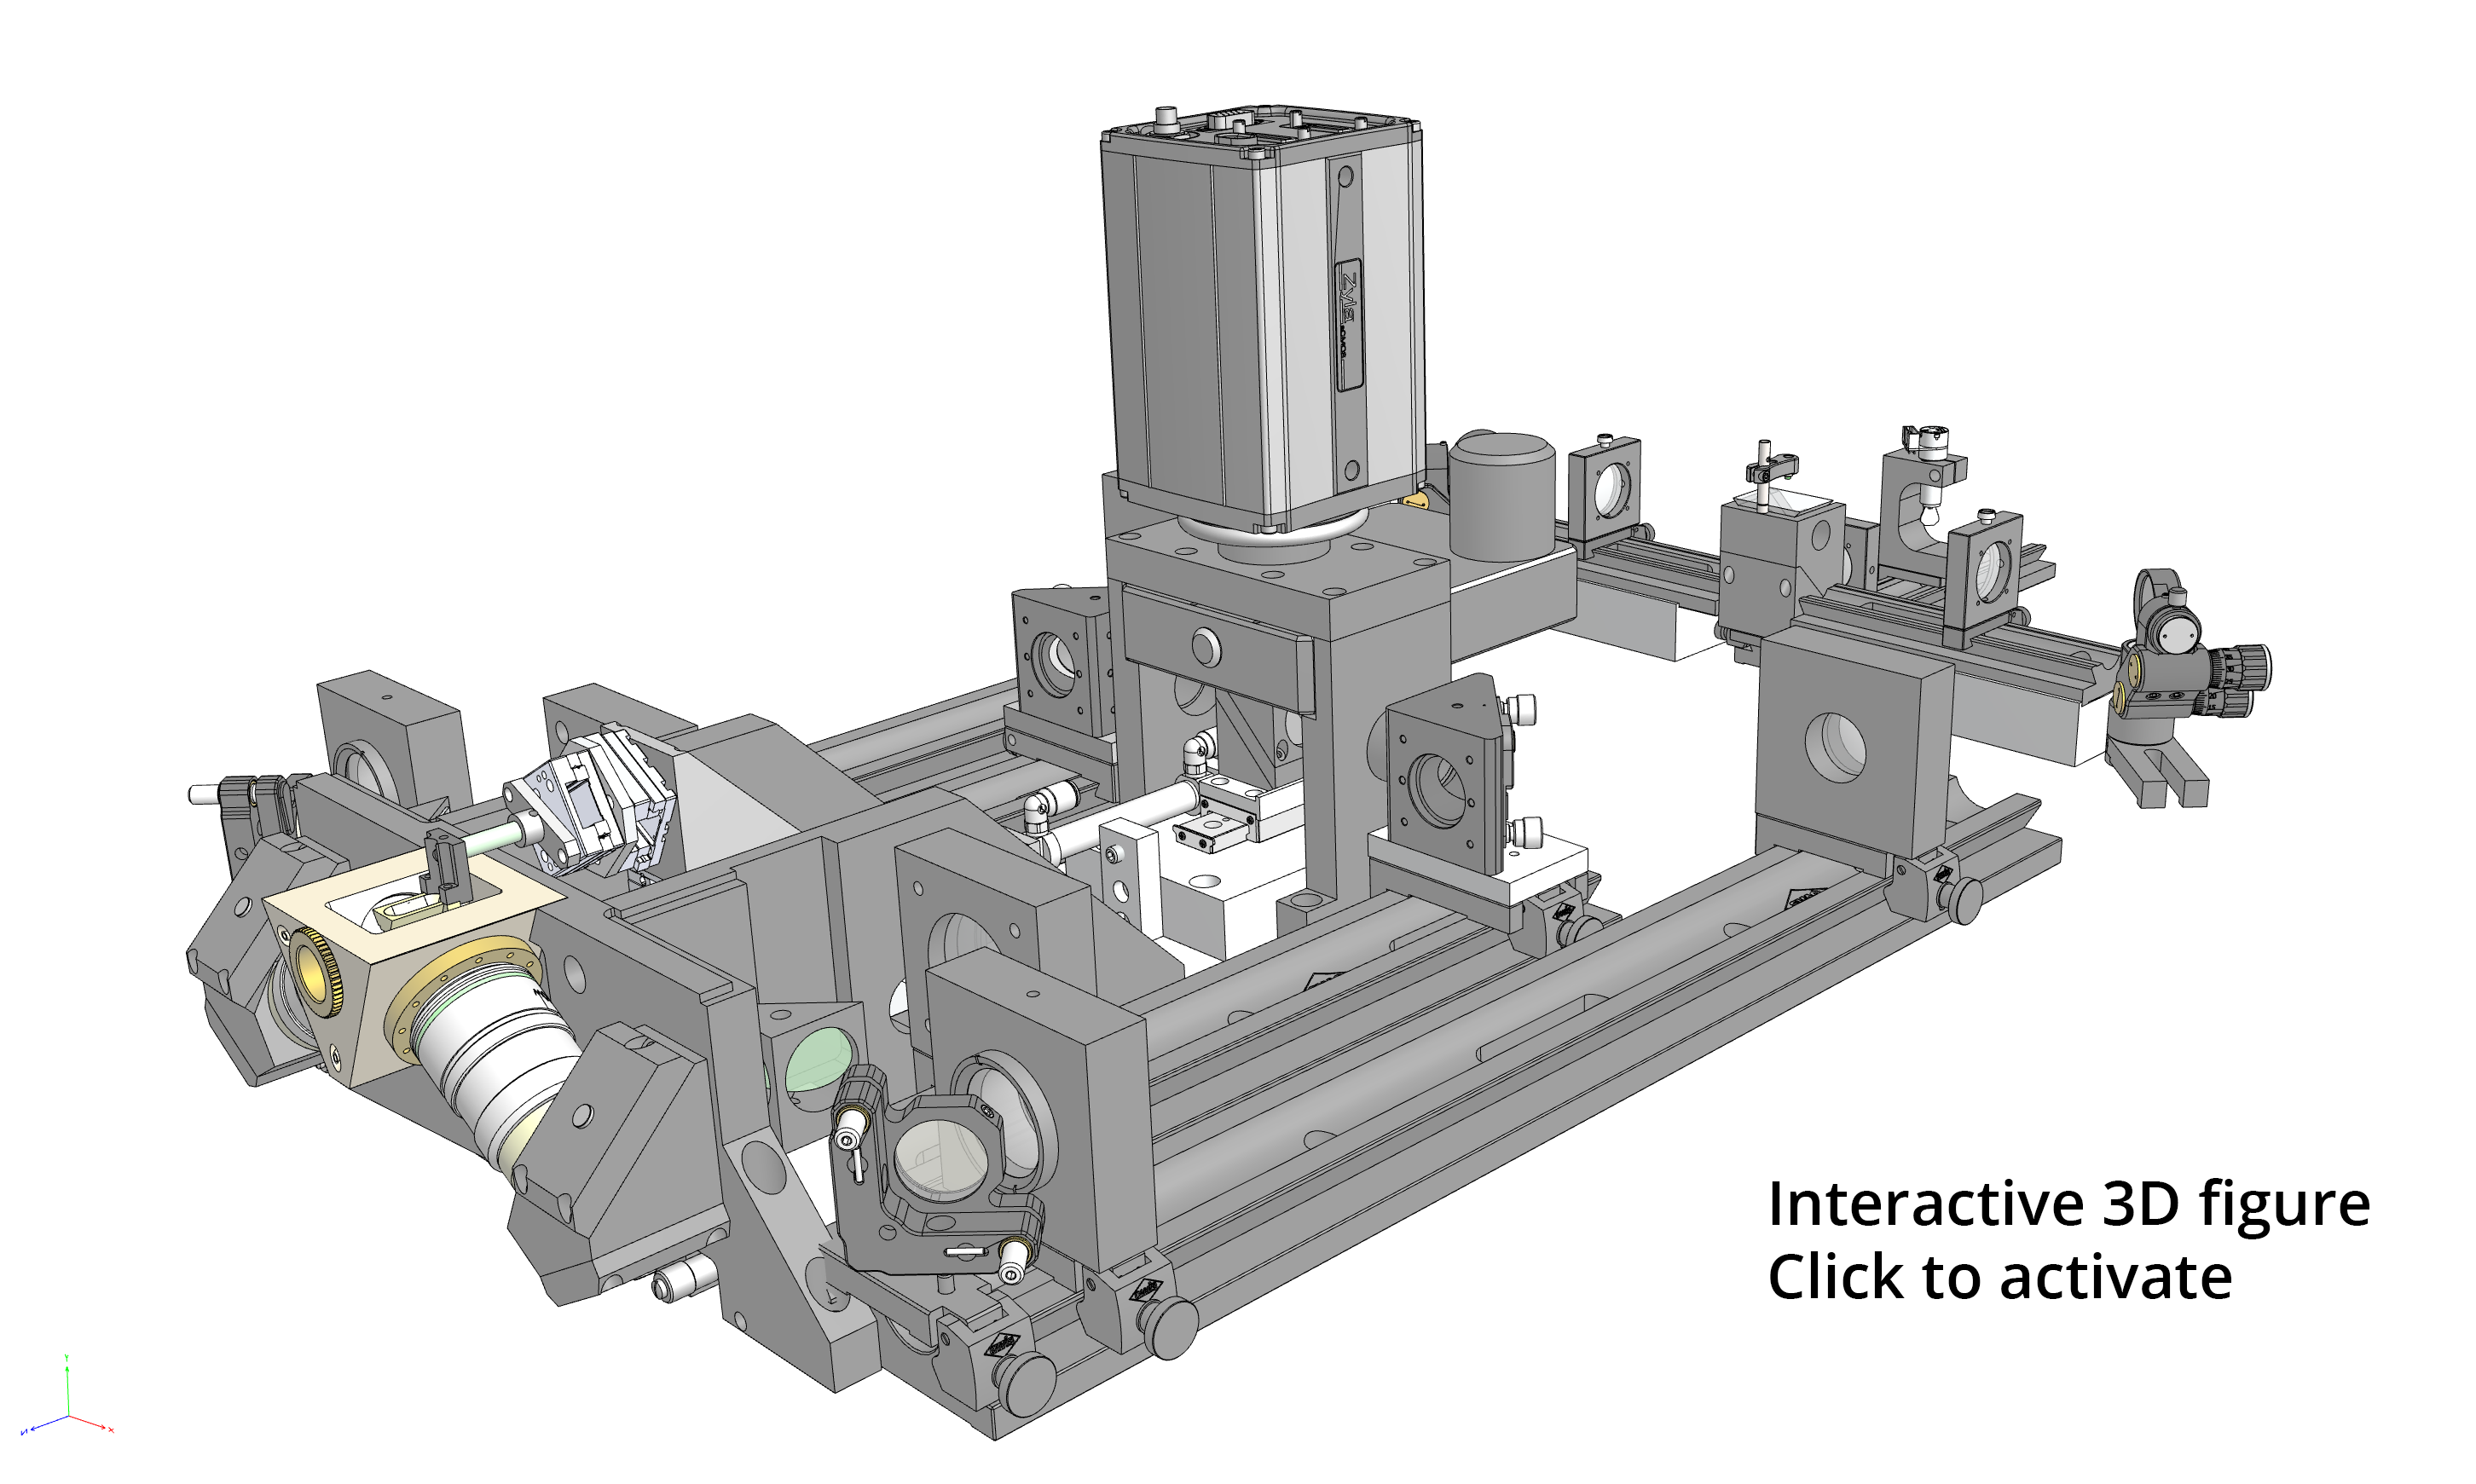
\includegraphics{DualMouseSPIM_beamScanning_forAppendix.png}}{DualMouseSPIM_beamScanning_forAppendix.prc}
  \bcaption[3D model of DualMouse-SPIM]{}
  \label{fig:splitter}
\end{figure}


\end{landscape}
